\documentclass[12pt]{article}
\usepackage[english]{babel}
\usepackage[utf8]{inputenc} 
\usepackage[T1]{fontenc}
\usepackage{graphicx}
\usepackage{amsmath}
\usepackage{wrapfig}
\usepackage{enumerate}
\usepackage[top=1in, bottom=1.25in, left=1.1in, right=1.1in]{geometry}
\usepackage[dvipsnames]{xcolor}
\usepackage{subcaption}

\begin{document}

\begin{titlepage}

\newcommand{\HRule}{\rule{\linewidth}{0.5mm}} 

\center 

\textsc{\LARGE Universidad de Sonora}\\[1.5cm]
\textsc{\Large Licenciatura en Física}\\[0.5cm]
\textsc{\large Física Computacional I}\\[0.5cm]

\HRule \\[0.4cm]
{\huge \bfseries Actividad 10 - Teoría del Caos y el Mapeo Logístico}\\[0.4cm] 
\HRule \\[1.5cm]

\begin{minipage}{0.4\textwidth}
\begin{flushleft} \large
\emph{Alumno:}\\
José Gabriel Navarro I.
\end{flushleft}
\end{minipage}
~
\begin{minipage}{0.4\textwidth}
\begin{flushright} \large
\emph{Profesor:} \\
Carlos Lizarraga Celaya
\end{flushright}
\end{minipage}\\[2cm]

18 de Mayo de 2018


\includegraphics[width=0.4\textwidth]{logo.png}\\
 
\vfill

\end{titlepage}

\section{Introducción}
En el presente reporte se habla acerca de la décima actividad realizada para la clase de Física Computacional I, el cual abarca el análisis del articulo de Geoff Boeing acerca de la Teoría del Caos y el Mapeo Logístico usando Python. Sin embargo, solamente se utilizo la información presentada en el blog, ya que para reproducir las graficas se utilizo el Sistema Algebraico wxMaxima.  \\

Se presenta en general una síntesis del blog de Geoff Boeing, en donde se habla acerca de las distintas características de un Sistema no-lineal Dinámico y mas específicamente de los sistemas caóticos, apoyándose en la idea del crecimiento poblacional por distintas generaciones. Para apoyar esta información, también se muestran las graficas que se reproducieron en wxMaxima que muestran claramente en que consisten este tipo de fenómenos. 

\section{Síntesis -  Teoría del Caos y el Mapeo Logístico}
La teoría del Caos es una rama de las matemáticas que analiza los sistemas no-lineales dinámicos. Es decir, un sistema que cambia conforme el tiempo pasa y que por factores multiplicativos, el sistema se vuelve mas complicado. \\

Los sistemas caóticos son un simple subtipo de sistemas no-lineales dinámicos. Pueden contener muy pocas partes con las que se pueda interactuar y pueden seguir reglas para nada complicadas, pero estos sistemas son muy dependientes en sus condiciones iniciales. Conforme el tiempo pasa, estos sistemas pueden producir resultados impredecibles o muy divergentes. 

\subsection{El Mapa Logístico}
El caos puede ser ejemplificado fácilmente utilizando el famoso mapa logístico. Este mapa esta basado en la curva mas común que muestra como la población crece lentamente, luego rápidamente, hasta que llega a su capacidad constante. El mapa logístico es llamado así porque gráfica la población en cualquier paso de tiempo contra su valor en el próximo tiempo, donde utiliza una ecuación diferencial no-lineal que toma pasos de tiempo discretos:

\centerline{$x_{t+1} = r x_t (1-x_t)$}
$     $

Esta ecuación define como va a funcionar nuestro sistema: x representa la población en cualquier tiempo t, y r representa la taza de crecimiento. En otras palabras, la población en cualquier tiempo es una función de la taza de crecimiento y nivel de población a un tiempo interior. A continuación se presenta varios aspectos de esta ecuación y las graficas obtenidas mediante wxMaxima de este modelo.

\subsection{Comportamiento del sistema y atractores}
A continuación se presenta una gráfica donde se muestran varias generaciones de poblaciones con distintas tazas de crecimiento:

\begin{figure}[h!]
    \centering
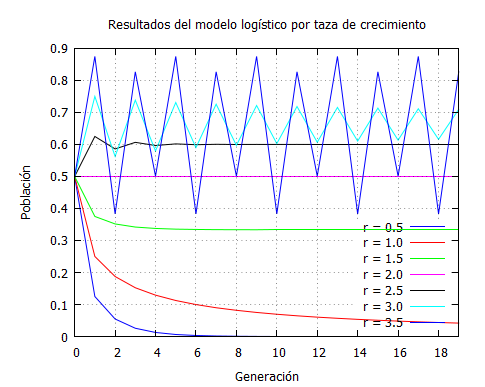
\includegraphics[width=4.5in]{DTaza.png}
\end{figure}

Como se puede observar, la población cambia conforme pasa el tiempo dadas distintas distintas tazas de crecimiento. Las tazas con valores muy pequeños rápidamente caen a 0, lo cual significa que la población muere. Para el valor de $r=2$, se tiene que esta se queda con un valor constante de población de 0.5. Las mas interesantes son las que tiene valores iguales a 3 y 3.5, ya que estas no mueren ni convergen a un valor, si no que parece que varia entre sus valores. \\

Un atractor es el valor, o el conjunto de valores, que el sistema toma después de un tiempo. Cuando el valor de la taza de crecimiento es pequeño, se tiene un atractor de punto fijo, mientras que para valores grandes, el sistema oscila entre 4 valores. A esto se le llama ciclo limite. Pero para aun valores mas grandes de la taza de crecimiento, empezamos a notar mas caos en los resultados, para esos casos, su atractor es mas extraño, como mas adelante podremos observar. \\

Para realizar esta gráfica en wxMaxima, se realizaron varios archivos con distintos valores de r (los mostrados en la gráfica), utilizando la misma condición inicial. Para crearlos, se utilizo un ciclo DO que permitió calcular el valor de la población para cada generación conforme pasa el tiempo. Una vez que se obtuvieron los archivos, estos se almacenaron en una variable y con ayuda de 2dplot y su función de "discrete" se graficaron los valores correspondientes a cada taza de crecimiento.

\subsection{Bifurcaciones y el Camino al Caos}
Para mostrar mejor los cambios que hay entre los cambios de la taza de crecimiento, vamos a tomar 200 generaciones de poblaciones y hacerlas variar entre 1000 tazas de crecimiento entre 0 y 4. Para visualizarlo se utiliza los diagramas de bifurcación. Estos diagramas son un resumen visual de la sucesión de los valores de la población mientras r aumenta.

\begin{figure}[h!]
    \centering
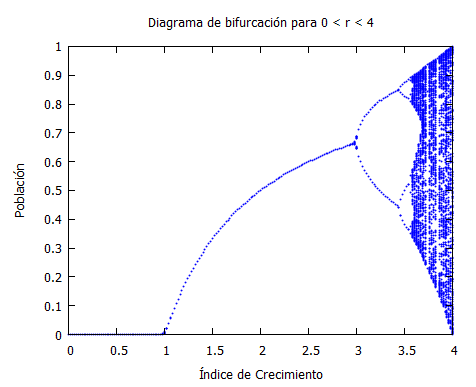
\includegraphics[width=4in]{Bif1.png}
\end{figure}

Para realizar todas estas graficas y las que presentan mas adelante, se utilizo un paquete nuevo de wxMaxima llamado Dynamics. Este paquete permite generar datos y simultáneamente graficarlos dependiendo de la función que se utilice. En este caso se utilizo la función "orbits", que permite realizar este tipo de graficas dando en su argumento el intervalo de iteraciones que va realizar y la función a evaluar. \\

Observando la gráfica podemos ver que para valores menores de 1, el sistema siempre colapsa a cero, es decir, se extingue la población. Para los valores de la taza de crecimiento entre 1 y 3, el sistema siempre se asienta en una población estable. Pero para algunos valores de r, como para 3.9 el diagrama muestra 100 valores diferentes, es decir, un valor diferente para cada una de sus 100 generaciones, no esta en un punto fijo. \\

\begin{figure}[h!]
    \centering
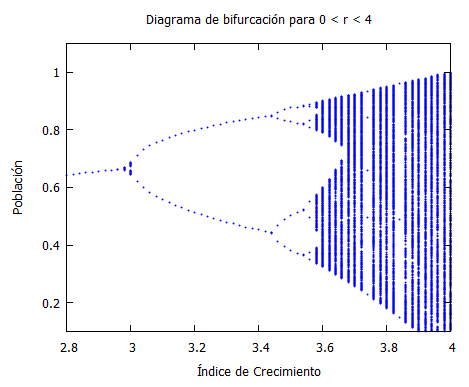
\includegraphics[width=3.5in]{Bif2.png}
\end{figure}

Acercándonos al intervalo entre 2.8 y 4, podemos observar como la posible población esta en dos caminos discretos. El sistema oscila entre dos valores, uno entre 0.5 y entre 0.8. En otras palabras, en esa taza de crecimiento, aplicando la ecuación logística a uno de esos valores, se obtiene el otro. Por eso llama diagrama de bifurcación. Después de $r=3.4$ podemos observar como el diagrama se parte ahora en 4 caminos. Luego de $r=3.5$ se divide de nuevo a 8 caminos. Esto es consistente con lo que se observo en la primera gráfica presentada, donde los valores de la población variaban dependiendo de su valor inicial y el valor de r que se le daba.

\subsection{El comienzo del Caos}
Después de la taza de crecimiento de 3.6, las bifurcaciones aumentan hasta que el sistema es capaz de caer en cualquier valor de población. Esto es conocido como bifurcación periodo-doble. Esto significa que mientras mas cambiamos el parámetro r, el mapa logístico oscilara en dos, luego cuatro, luego ocho, luego 16, luego 32 (y así sucesivamente)  valores para la población.

\begin{figure}[h!]
    \centering
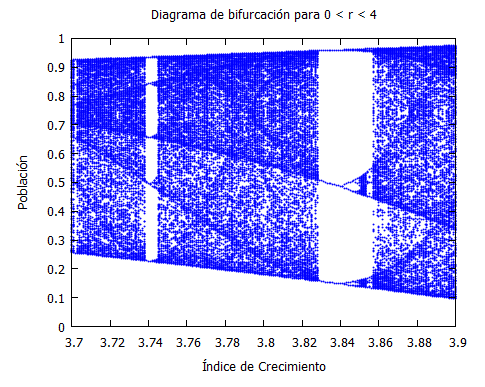
\includegraphics[width=3.5in]{Bif3.png}
\end{figure}

Cuando alcanzamos valores mas altos, como de 3.9, habrá bifurcado tanto que el sistema parece saltar de una manera aleatoria entre todos los valores que puede tomar la población. Sin embargo, si realizamos una acercamiento entre 3.7 y 3.9, podemos observar como se puede notar un patrón parecido al que ya habiamos visto anteriormente. De todo el caos que se observa, el sistema vuelve a poner en orden, con solo 3 ramas de bifurcación. Esto es el caos, determinista y aperiódico. 

\subsection{Fractales y Atractores Extraños}
En la gráfica anterior podemos observar como las bifurcaciones en la taza de 3.85 parece familiar. Si hacemos un acercamiento, podemos ver exactamente la misma estructura que se veía a un nivel macro. Y si hacemos mas acercamientos, podremos ver exactamente el mismo patrón para escalas mas finas infinitamente. Esto se debe a que los sistemas caóticos tienen atractores extraños, los cuales pueden ser caracterizados como fractales. Esto significa que son similares entre ellos, es decir que tienen la misma estructura a cualquier escala, como lo es el caso del presente ejemplo.

\begin{figure}[h!]
    \centering
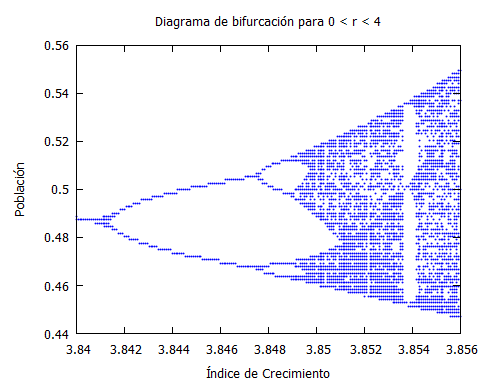
\includegraphics[width=4in]{Bif4.png}
\end{figure}

Otra forma de visualizar esto es con un diagrama de fase (Gráfica de Poincaré), la cual gráfica la población de una generación t+1 en el eje y, contra la población en el valor t en el eje de las x. Dependiendo del valor que se le de a la r, puede que no se difracte, mostrando solo un punto, lo cual significa que el valor de la población es constante. Ahora bien si aparecen mas puntos, significa que la población puede tener varios valores, por ejemplo:

\begin{figure}[h!]
\begin{subfigure}{.5\textwidth}
  \centering
  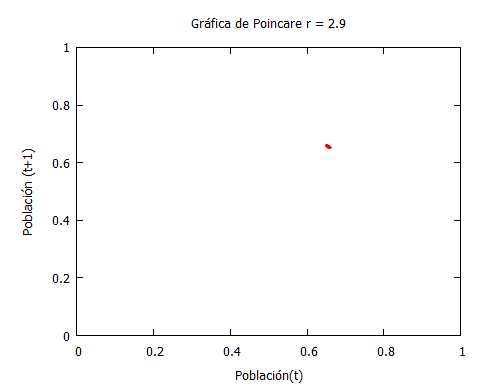
\includegraphics[width=.7\linewidth]{Poi1.png}
  \caption{r = 2.9}
  \label{fig:sfig1}
\end{subfigure}%
\begin{subfigure}{.5\textwidth}
  \centering
  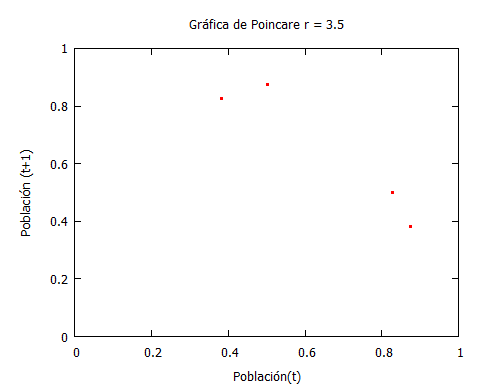
\includegraphics[width=.7\linewidth]{Poi2.png}
  \caption{r = 3.5}
  \label{fig:sfig2}
\end{subfigure}
\end{figure}

Pero si este tiene varias difracciones, se muestra una serie de puntos que forman una parábola. Si se grafican todos los valores de r con sus posibles difracciones, se llega a un patrón de parábolas que no se sobreponen. A estos valores se le conocen como el régimen caótico, donde el mapa logístico se comporta de manera caótica.

\begin{figure}[h!]
\begin{subfigure}{.6\textwidth}
  \centering
  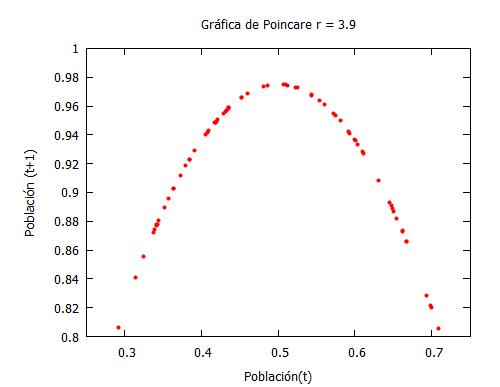
\includegraphics[width=.8\linewidth]{Poi3.png}
  \caption{r = 3.9}
  \label{fig:sfig1}
\end{subfigure}
\begin{subfigure}{.6\textwidth}
  \centering
  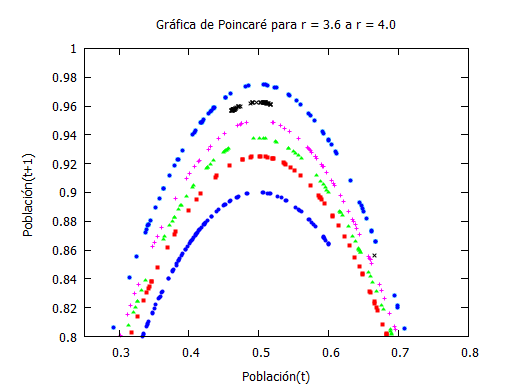
\includegraphics[width=.8\linewidth]{Poi4.png}
  \caption{3.6 < r < 4.0 }
  \label{fig:sfig2}
\end{subfigure}
\end{figure}

Para realizar estas graficas se realizo utilizando otro ciclo DO, pero en este se calculaba el valor de la población, y en el mismo ciclo se calculaba el valor siguiente y se mandaban aun archivo. Con esto, solamente se graficaron con 2d plot de igual manera que la grafica presentada al inicio. 
\subsection{Caos VS Aleatoriedad}
A veces es muy difícil diferenciar si ciertas series de tiempo son caóticas o solamente son números aleatorios cuando no entiendes totalmente lo que contiene los sistemas dinámicos. Por ejemplo:

\begin{figure}[h!]
    \centering
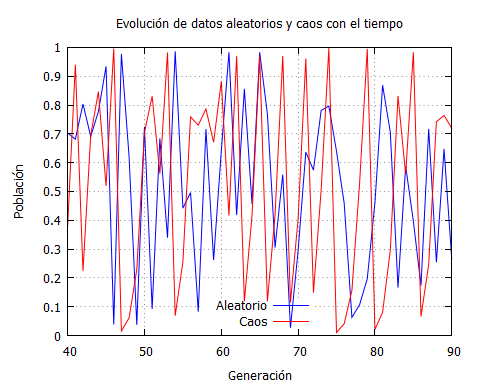
\includegraphics[width=3.4in]{cva.png}
\end{figure}

Ambas lineas parece que solamente cambian de valores rápidamente. La linea azul si representa datos aleatorios, pero la otra linea representa nuestro modelo logístico cuando nuestro crecimiento de taza es de 3.99, el cual es caos determinista. Para diferenciarlos se pueden utilizar los diagramas de fase, donde como se puede observar, los puntos azules solamente representan ruido, mientras que los rojos muestran la parábola de la que ya se había hablado antes. 

\begin{figure}[h!]
    \centering
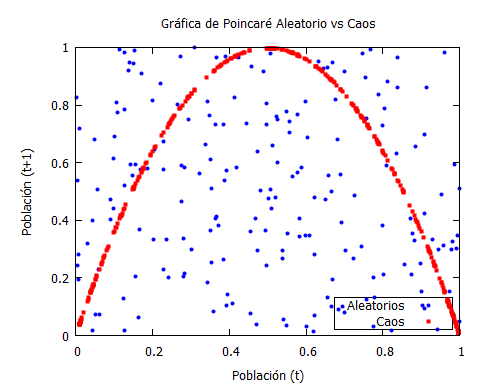
\includegraphics[width=4in]{Poi5.png}
\end{figure}

\subsection{El Efecto Mariposa}
Los sistemas caóticos también se caracterizan por ser muy sensibles a los cambios en sus condiciones iniciales. Como su atractor es raro, los puntos que están cercanos, divergen con el tiempo. Esto hace que modelar fenómenos en la vida real y predecir esto fenómenos se vuelva difícil, porque si desde un inicio los parámetros no son medidos con precisión, estos pequeños errores se hacen grandes conforme pasa el tiempo. \\

Por ejemplo, en la siguiente imagen podemos ver que ambos tienen la misma taza de crecimiento, 3.9. La linea representa una población inicial de 0.5, y la roja de 0.50001. A pesar de tener condiciones iniciales muy parecidas, conforme pasa el tiempo, divergen. En las primeras generaciones si se puede observar que los resultados son iguales, pero después de ello, cambian dramáticamente.

\pagebreak

\begin{figure}[h!]
    \centering
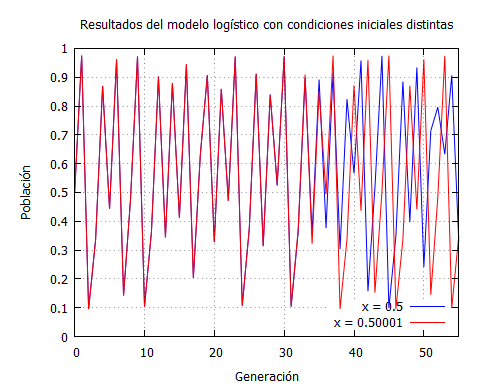
\includegraphics[width=5in]{CI.png}
\end{figure}

Esto es conocido como el efecto mariposa: una mariposa aletea sus alas en China, y en Texas aparece un tornado. Pequeños eventos pueden causar errores fatales y alterar el futuro del estudio. 

\subsection{Las implicaciones del Caos}
Los sistemas caóticos y sistemas fractales pueden presentarse en la vida real, y se ha observado ya en fugas de tubos, frecuencias del corazón y generadores aleatorios de números. Muchos científicos han estudiado las implicaciones de la teoría del caos en otras áreas como las ciencias sociales, ciudades y plantación urbana, pero el caos en general indica una cosa. El caos fundamentalmente indica que hay limites para el conocimiento y predicción, algunos futuros pueden ser desconocidos, no importa la presición que tengas. 

\section{Conclusión}
Gracias a esta práctica, solo queda mas en claro el poder que tienen los Sistemas Algebraicos Computacionales, para ser mas específicos wxMaxima. Poder recrear tanto cálculos como graficas que se realizan originalmente en Python es increíble. Además de que no solo realizo la mayoría del trabajo que pudo hacer Python, si no que el tema del que se hablo también es muy interesante y no algo muy fácil de asimilar solamente leyendo. \\
 
Como ya había mencionado anteriormente, es muy importante aprender el uso y manejo de este programa ya que puede ayudarnos no solamente ahora en nuestra carrera como estudiante, sino también ya en nuestra carrera como científicos. Este tema me pareció muy interesante, entretenido y un buen cierre para lo que viene siendo la ultima practica del curso. 

\section{Bibliografía empleada}
\begin{itemize}
    \item Bifurcation Diagram. (2016). Recuperado de: www.vanderbilt.edu/AnS/psychology\\/cogsci/chaos/workshop/BD.html
    \item Plotting. (8 de Octubre de 2012). Recuperado de: cs.swan.ac.uk\\/\~csoliver/ok-sat-library/internet\_html/doc/doc/Maxima/5.27.0/html/maxima\_12.html
    \item Chaos Theory and the Logistic Map. (25 de Marzo de 2015). Recuperado de: geoffboeing.com/2015/03/chaos-theory-logistic-map/
    \item Chaotic dynamics with Maxima. (16 de Enero de 2013). Recuperado de: arxiv.org/pdf\\/1301.3240.pdf
\end{itemize}

\end{document}